\section{Reading Motion Graphs}
\label{sec:graphs}

We have drawn a velocity--time graph whenever we needed one (Figures~\ref{fig:vtgraph} and~\ref{fig:thrown}) and a displacement--time graph once (Figure~\ref{fig:vtgraph}(b)). It is time to be systematic. Any motion along a line can be drawn three ways, as position against time, velocity against time, and acceleration against time, and the three graphs are not independent: each can be built from the one beside it. Moving between them, in both directions, is the graphical form of everything in this chapter, and it is a skill you will use in every later chapter that involves motion. Hewitt gives the reading rules in his appendix on graphing; here we practise them on one motion drawn all three ways.

Figure~\ref{fig:threegraphs} shows a tram pulling away from one stop and drawing up at the next. The tram starts from rest, speeds up steadily for \SI{8}{\second}, holds a constant velocity for \SI{12}{\second}, then brakes steadily to a halt in \SI{4}{\second}. Read the three panels from the middle outward. Panel~(b), the velocity--time graph, is the one to start with, because its slope gives panel~(c) and its area gives panel~(a).

\begin{figure}[htb]
\centering
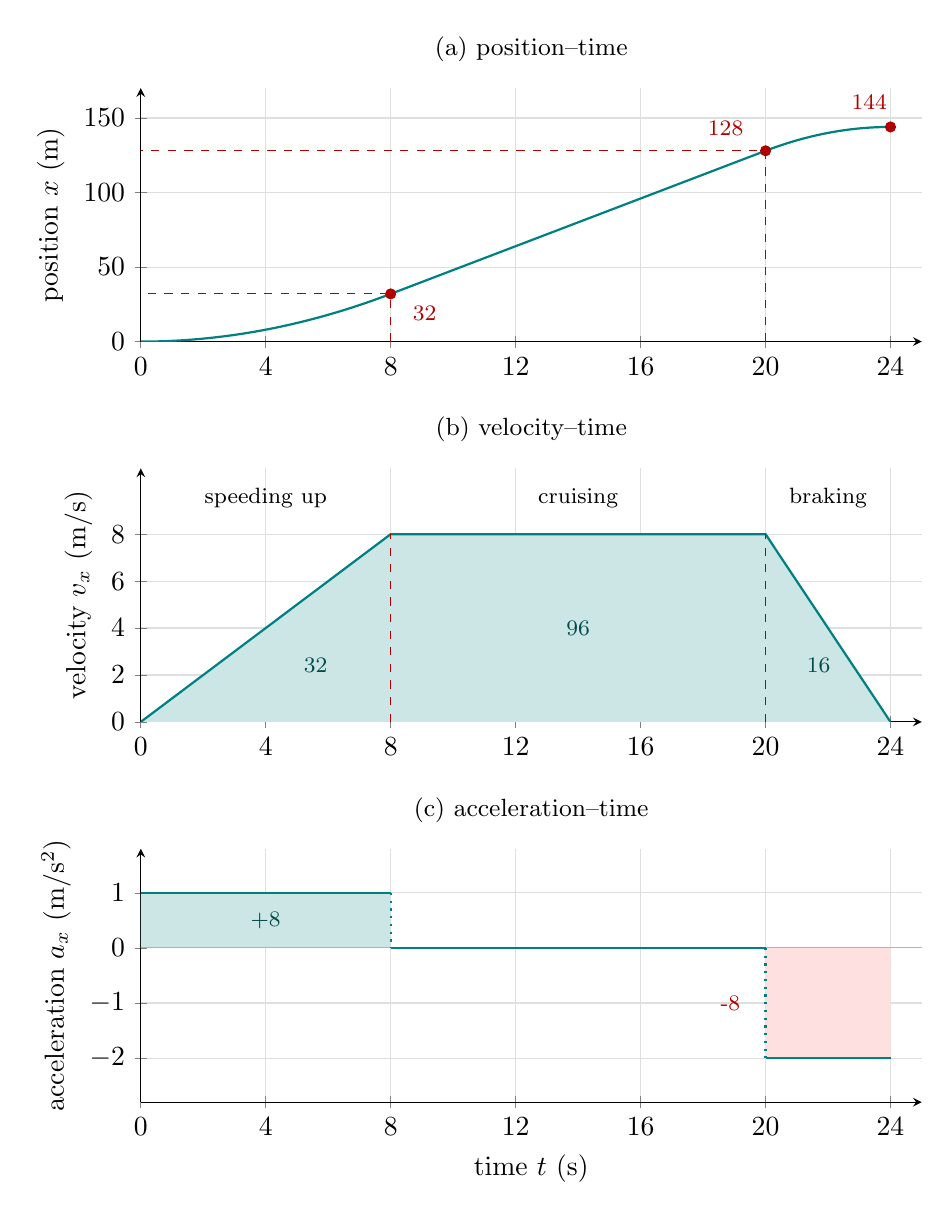
\begin{tikzpicture}
\begin{axis}[
  name=xt,
  width=11.5cm,height=4.8cm,
  ylabel={position $x$ (m)},
  xmin=0,xmax=25,ymin=0,ymax=170,
  xtick={0,4,...,24},ytick={0,50,100,150},
  grid=major,grid style={gray!25},
  axis lines=left,
  title={(a) position--time},title style={font=\small},
]
\addplot[teal,thick,domain=0:8,samples=40] {0.5*x^2};
\addplot[teal,thick,domain=8:20,samples=2] {32+8*(x-8)};
\addplot[teal,thick,domain=20:24,samples=40] {128+8*(x-20)-(x-20)^2};
\draw[dashed,red!70!black] (axis cs:8,0) -- (axis cs:8,32) -- (axis cs:0,32);
\draw[dashed,red!70!black] (axis cs:20,0) -- (axis cs:20,128) -- (axis cs:0,128);
\addplot[only marks,mark=*,mark size=1.8pt,red!70!black] coordinates {(8,32) (20,128) (24,144)};
\node[red!70!black,font=\footnotesize,anchor=north west] at (axis cs:8.4,30) {\SI{32}{\metre}};
\node[red!70!black,font=\footnotesize,anchor=south east] at (axis cs:19.6,132) {\SI{128}{\metre}};
\node[red!70!black,font=\footnotesize,anchor=south east] at (axis cs:24.2,149) {\SI{144}{\metre}};
\end{axis}
\begin{axis}[
  name=vt,
  at={(xt.below south west)},anchor=above north west,yshift=-3mm,
  width=11.5cm,height=4.8cm,
  ylabel={velocity $v_x$ (m/s)},
  xmin=0,xmax=25,ymin=0,ymax=10.8,
  xtick={0,4,...,24},ytick={0,2,4,6,8},
  grid=major,grid style={gray!25},
  axis lines=left,
  title={(b) velocity--time},title style={font=\small},
]
\addplot[fill=teal!20,draw=none] coordinates {(0,0) (8,8) (20,8) (24,0)} \closedcycle;
\addplot[teal,thick] coordinates {(0,0) (8,8) (20,8) (24,0)};
\draw[dashed,red!70!black] (axis cs:8,0) -- (axis cs:8,8);
\draw[dashed,red!70!black] (axis cs:20,0) -- (axis cs:20,8);
\node[teal!60!black,font=\footnotesize] at (axis cs:5.6,2.4) {\SI{32}{\metre}};
\node[teal!60!black,font=\footnotesize] at (axis cs:14,4) {\SI{96}{\metre}};
\node[teal!60!black,font=\footnotesize] at (axis cs:21.7,2.4) {\SI{16}{\metre}};
\node[font=\footnotesize,anchor=south] at (axis cs:4,8.7) {speeding up};
\node[font=\footnotesize,anchor=south] at (axis cs:14,8.7) {cruising};
\node[font=\footnotesize,anchor=south] at (axis cs:22,8.7) {braking};
\end{axis}
\begin{axis}[
  name=at,
  at={(vt.below south west)},anchor=above north west,yshift=-3mm,
  width=11.5cm,height=4.8cm,
  xlabel={time $t$ (s)},ylabel={acceleration $a_x$ (m/s$^2$)},
  xmin=0,xmax=25,ymin=-2.8,ymax=1.8,
  xtick={0,4,...,24},ytick={-2,-1,0,1},
  grid=major,grid style={gray!25},
  axis lines=left,
  title={(c) acceleration--time},title style={font=\small},
]
\addplot[fill=teal!20,draw=none] coordinates {(0,0) (0,1) (8,1) (8,0)} \closedcycle;
\addplot[fill=red!12,draw=none] coordinates {(20,0) (20,-2) (24,-2) (24,0)} \closedcycle;
\draw[gray!60] (axis cs:0,0) -- (axis cs:25,0);
\addplot[teal,thick] coordinates {(0,1) (8,1)};
\addplot[teal,thick] coordinates {(8,0) (20,0)};
\addplot[teal,thick] coordinates {(20,-2) (24,-2)};
\draw[teal,thick,dotted] (axis cs:8,1) -- (axis cs:8,0);
\draw[teal,thick,dotted] (axis cs:20,0) -- (axis cs:20,-2);
\node[teal!60!black,font=\footnotesize] at (axis cs:4,0.5) {\SI{+8}{\metre\per\second}};
\node[red!70!black,font=\footnotesize,anchor=east] at (axis cs:19.5,-1) {\SI{-8}{\metre\per\second}};
\end{axis}
\end{tikzpicture}
\caption{One tram ride drawn three ways, on a shared time axis. (a) Position: a parabola bending upward while the tram speeds up, a straight line while it cruises, and a parabola bending over as it brakes, ending level at \SI{144}{\metre}. (b) Velocity: the slope of (a). The shaded trapezium is the displacement, cut by the dashed lines into \SI{32}{\metre}, \SI{96}{\metre}, and \SI{16}{\metre}. (c) Acceleration: the slope of (b). The areas under it, $+\SI{8}{\metre\per\second}$ and $-\SI{8}{\metre\per\second}$, are the velocity gained and lost, and they cancel because the tram ends at rest.}
\label{fig:threegraphs}
\end{figure}

\begin{twoviews}{translating between the three graphs}
\elem Going \emph{down} the stack, from position to velocity to acceleration, means taking slopes. The slope of the position--time graph at an instant is the velocity then; where the graph is curved, lay a ruler along the curve so that it touches at just that point (a \emph{tangent}) and read the rise over the run. The slope of the velocity--time graph is the acceleration; where that graph is made of straight segments, as in Figure~\ref{fig:threegraphs}(b), the acceleration is constant on each segment and jumps between them. Going \emph{up} the stack means taking areas. The area under the acceleration--time graph between two instants is the change in velocity; the area under the velocity--time graph is the change in position. Areas below the axis count as negative. When the graphs are made of straight lines, every area is a rectangle, a triangle, or a trapezium.

\calc The three panels are the graphs of $x(t)$, $v_x(t) = \dd x/\dd t$, and $a_x(t) = \dd v_x/\dd t$. Going down the stack is differentiation; going up is integration, with the starting value supplied separately: $v_x(t) = v_x(0) + \int_0^t a_x\,\dd t'$ and $x(t) = x(0) + \int_0^t v_x\,\dd t'$. The sign of the second derivative tells you how the position graph bends: where $a_x > 0$ the position--time curve is \emph{concave up} (it bends like a smile), where $a_x < 0$ it is \emph{concave down}, and where $a_x = 0$ it is straight. A corner in the velocity graph, where the slope changes abruptly, is a jump in the acceleration graph. A corner in the position graph would be a jump in velocity, which needs an infinite acceleration and does not happen to real trams.
\end{twoviews}

\begin{keyidea}[How to read the three graphs]
\begin{center}
\renewcommand{\arraystretch}{1.3}
\small
\begin{tabular}{llll}
\toprule
graph & its slope is & the area under it is & shape when $a_x$ is constant \\
\midrule
position--time $x(t)$ & velocity $v_x$ & & parabola (a line if $a_x = 0$) \\
velocity--time $v_x(t)$ & acceleration $a_x$ & change in position $\Delta x$ & straight line \\
acceleration--time $a_x(t)$ & & change in velocity $\Delta v_x$ & horizontal line \\
\bottomrule
\end{tabular}
\end{center}
\elemtag\ Slopes are rise over run; areas are counted in rectangles, triangles, and trapezia, negative below the axis. \calctag\ Slopes are derivatives and areas are integrals, and the two operations undo each other, which is why the stack can be read in either direction.
\end{keyidea}

\begin{example}{Three graphs of one tram ride}{tramgraphs}
Use the velocity--time graph in Figure~\ref{fig:threegraphs}(b) to find (a) the tram's acceleration during each of the three phases, (b) how far apart the two stops are, and (c) the tram's average velocity for the whole trip. Then (d) explain the shape of each piece of the position--time graph in panel~(a).

\elem (a) Acceleration is the slope of the velocity--time graph. From $t = 0$ to \SI{8}{\second} the line rises from $0$ to \SI{8.0}{\metre\per\second}: slope $(\SI{8.0}{\metre\per\second})/(\SI{8}{\second}) = \SI{1.0}{\metre\per\second\squared}$. From \SI{8}{\second} to \SI{20}{\second} the line is horizontal: slope zero, no acceleration. From \SI{20}{\second} to \SI{24}{\second} the line falls from \SI{8.0}{\metre\per\second} to $0$: slope $(\SI{-8.0}{\metre\per\second})/(\SI{4}{\second}) = \SI{-2.0}{\metre\per\second\squared}$. The tram brakes twice as hard as it accelerates. These three values are exactly what panel~(c) shows.

(b) Displacement is the area under the velocity--time graph. The region is a trapezium, and the dashed lines cut it into a triangle, a rectangle, and a triangle:
\[
\tfrac12(\SI{8}{\second})(\SI{8.0}{\metre\per\second}) + (\SI{12}{\second})(\SI{8.0}{\metre\per\second}) + \tfrac12(\SI{4}{\second})(\SI{8.0}{\metre\per\second}) = 32 + 96 + 16\ \si{\metre} = \SI{144}{\metre}.
\]
The stops are \SI{144}{\metre} apart, which is where panel~(a) ends.

(c) Average velocity is displacement over time: $\SI{144}{\metre}/\SI{24}{\second} = \SI{6.0}{\metre\per\second}$, less than the cruising velocity of \SI{8.0}{\metre\per\second} because the tram spends half the trip below cruising speed. On panel~(a) this is the slope of the chord from $(0, 0)$ to $(\SI{24}{\second}, \SI{144}{\metre})$.

(d) The slope of the position--time graph is the velocity. In the first phase the velocity grows, so the slope steepens and the curve bends upward; it is the parabola $x = \tfrac12 a t^2$ of Galileo's law, and its value at $t = \SI{8}{\second}$ is the \SI{32}{\metre} triangle from part~(b). In the cruising phase the velocity is fixed, so the graph is a straight line of slope \SI{8.0}{\metre\per\second}. In the braking phase the velocity shrinks, so the slope flattens and the curve bends over, arriving at the second stop with zero slope: the tram is at rest.

\calc Write the velocity as a piecewise function and integrate from $x(0) = 0$, in SI units:
\begin{align*}
0 \le t \le 8:&\quad v_x = (1.0)\,t, & x &= \tfrac12(1.0)\,t^2, & x(8) &= 32; \\
8 \le t \le 20:&\quad v_x = 8.0, & x &= 32 + 8.0\,(t - 8), & x(20) &= 128; \\
20 \le t \le 24:&\quad v_x = 8.0 - 2.0\,(t - 20), & x &= 128 + 8.0\,(t - 20) - (t - 20)^2, & x(24) &= 144.
\end{align*}
Differentiating each $v_x$ gives $a_x = 1.0$, $0$, and $-2.0\ \si{\metre\per\second\squared}$, part~(a); the last $x$ value is part~(b); and $\bar v_x = \frac{1}{24}\int_0^{24} v_x\,\dd t = 144/24 = \SI{6.0}{\metre\per\second}$ is part~(c). For part~(d), the second derivative of $x$ is $a_x$: positive on the first piece (concave up), zero on the second (straight), negative on the third (concave down). The first and third pieces are parabolas and the second is a line, and they join smoothly because $v_x = \dd x/\dd t$ is continuous, even though $a_x$ is not.

Sanity check: \SI{8}{\metre\per\second} is about \SI{29}{\kilo\metre\per\hour}, and \SI{144}{\metre} is a short city block, both reasonable for a hop between neighbouring stops. Notice that the position graph never comes back down, though the tram does stop: a level stretch of a position graph means \emph{at rest}, and a falling stretch would mean \emph{reversing}, neither of which happens here.\qed
\end{example}

\begin{example}{Reading a position--time graph}{xtgraph}
Now use only panel~(a) of Figure~\ref{fig:threegraphs}, the position--time graph, and pretend the other two panels are hidden. (a) Find the tram's velocity at $t = \SI{4}{\second}$, at $t = \SI{14}{\second}$, and at $t = \SI{22}{\second}$. (b) Find its acceleration at $t = \SI{4}{\second}$. (c) Without calculating anything, decide whether the tram ever moves backwards.

\elem (a) Velocity is the slope of the position--time graph. At $t = \SI{14}{\second}$ the graph is a straight line, so its slope is the same everywhere on that segment: between $t = \SI{8}{\second}$ ($x = \SI{32}{\metre}$) and $t = \SI{20}{\second}$ ($x = \SI{128}{\metre}$) the rise is \SI{96}{\metre} over a run of \SI{12}{\second}, giving \SI{8.0}{\metre\per\second}. At $t = \SI{4}{\second}$ the graph is curved, so we want the slope of the tangent there. A ruler laid against the curve at $t = \SI{4}{\second}$ passes through about $(\SI{2}{\second}, \SI{0}{\metre})$ and $(\SI{6}{\second}, \SI{16}{\metre})$, a slope of \SI{4.0}{\metre\per\second}. A cleaner method, which Worked Example~\ref{ex:diff} showed is exact for a parabola, is a short chord centred on the instant: reading $x(\SI{2}{\second}) = \SI{2}{\metre}$ and $x(\SI{6}{\second}) = \SI{18}{\metre}$ from the graph, the chord slope is $(18 - 2)/(6 - 2) = \SI{4.0}{\metre\per\second}$. At $t = \SI{22}{\second}$ the centred chord from $(\SI{20}{\second}, \SI{128}{\metre})$ to $(\SI{24}{\second}, \SI{144}{\metre})$ gives $16/4 = \SI{4.0}{\metre\per\second}$ again: the tram passes through \SI{4}{\metre\per\second} once while speeding up and once while braking.

(b) Acceleration is the rate at which the slope changes. The slope is zero at $t = 0$ (the tram starts from rest, and the curve leaves the origin flat), \SI{4.0}{\metre\per\second} at $t = \SI{4}{\second}$, and \SI{8.0}{\metre\per\second} at $t = \SI{8}{\second}$, where the curve joins the straight segment smoothly. The slope grows by \SI{4.0}{\metre\per\second} in each \SI{4}{\second}, so the acceleration is \SI{1.0}{\metre\per\second\squared}, matching Worked Example~\ref{ex:tramgraphs}.

(c) Moving backwards would mean $x$ decreasing, a stretch of the graph sloping downhill. There is none; the graph rises throughout and merely levels off at the end. The tram only ever moves forward, and at the end it stops.

\calc (a) On the first piece $x = \tfrac12(1.0)t^2$, so $v_x = \dd x/\dd t = (1.0)t = \SI{4.0}{\metre\per\second}$ at $t = \SI{4}{\second}$; the centred chord agreed exactly because for a quadratic, $[x(t+h) - x(t-h)]/2h = \dd x/\dd t$ for any $h$. On the middle piece $v_x = \dd x/\dd t = \SI{8.0}{\metre\per\second}$. On the last piece $v_x = 8.0 - 2.0(t - 20) = \SI{4.0}{\metre\per\second}$ at $t = \SI{22}{\second}$. (b) $a_x = \dd^2 x/\dd t^2 = \SI{1.0}{\metre\per\second\squared}$ on the first piece. (c) $x$ decreases only where $\dd x/\dd t < 0$, and $v_x \ge 0$ on every piece, reaching zero only at $t = 0$ and $t = \SI{24}{\second}$.

The lesson is that a position--time graph contains the same information as the other two, but you have to dig it out with slopes, once for velocity and twice for acceleration. The velocity--time graph is usually the most convenient of the three, because both of its neighbours are one step away.\qed
\end{example}

\begin{modelnote}[A graph is not a map]
The commonest mistake with motion graphs is to read them as pictures of the journey. The position--time graph in Figure~\ref{fig:threegraphs}(a) rises steadily to the right, but the tram did not climb a hill; it ran along level track, and the ``rise'' is the tram getting farther from the first stop as the clock runs. Likewise a velocity--time graph that slopes down, as in the braking phase, does not show the tram going downhill or backwards; it shows the velocity decreasing while the tram continues forward. The horizontal axis is always \emph{time}, and a point on the graph is the reading of an instrument (odometer, speedometer, or accelerometer) at that moment. Hewitt's graph of free fall makes the same point in reverse: the distance fallen, plotted against time, is a curve that bends \emph{upward}, even though the object is falling down. If you catch yourself imagining a graph as a track, switch to reading it as a table of numbers and ask what each column would say.
\end{modelnote}

\begin{checkbox}
The position--time graphs of two cyclists on the same road cross at $t = \SI{30}{\second}$. What do the two cyclists have in common at that instant, and what need they not have in common? Answer the same question for two velocity--time graphs that cross.
\end{checkbox}

